\documentclass[../main.tex]{subfiles}
\graphicspath{{\subfix{../images/}}}
\begin{document}


\begin{figure}[htb!]
\centering
  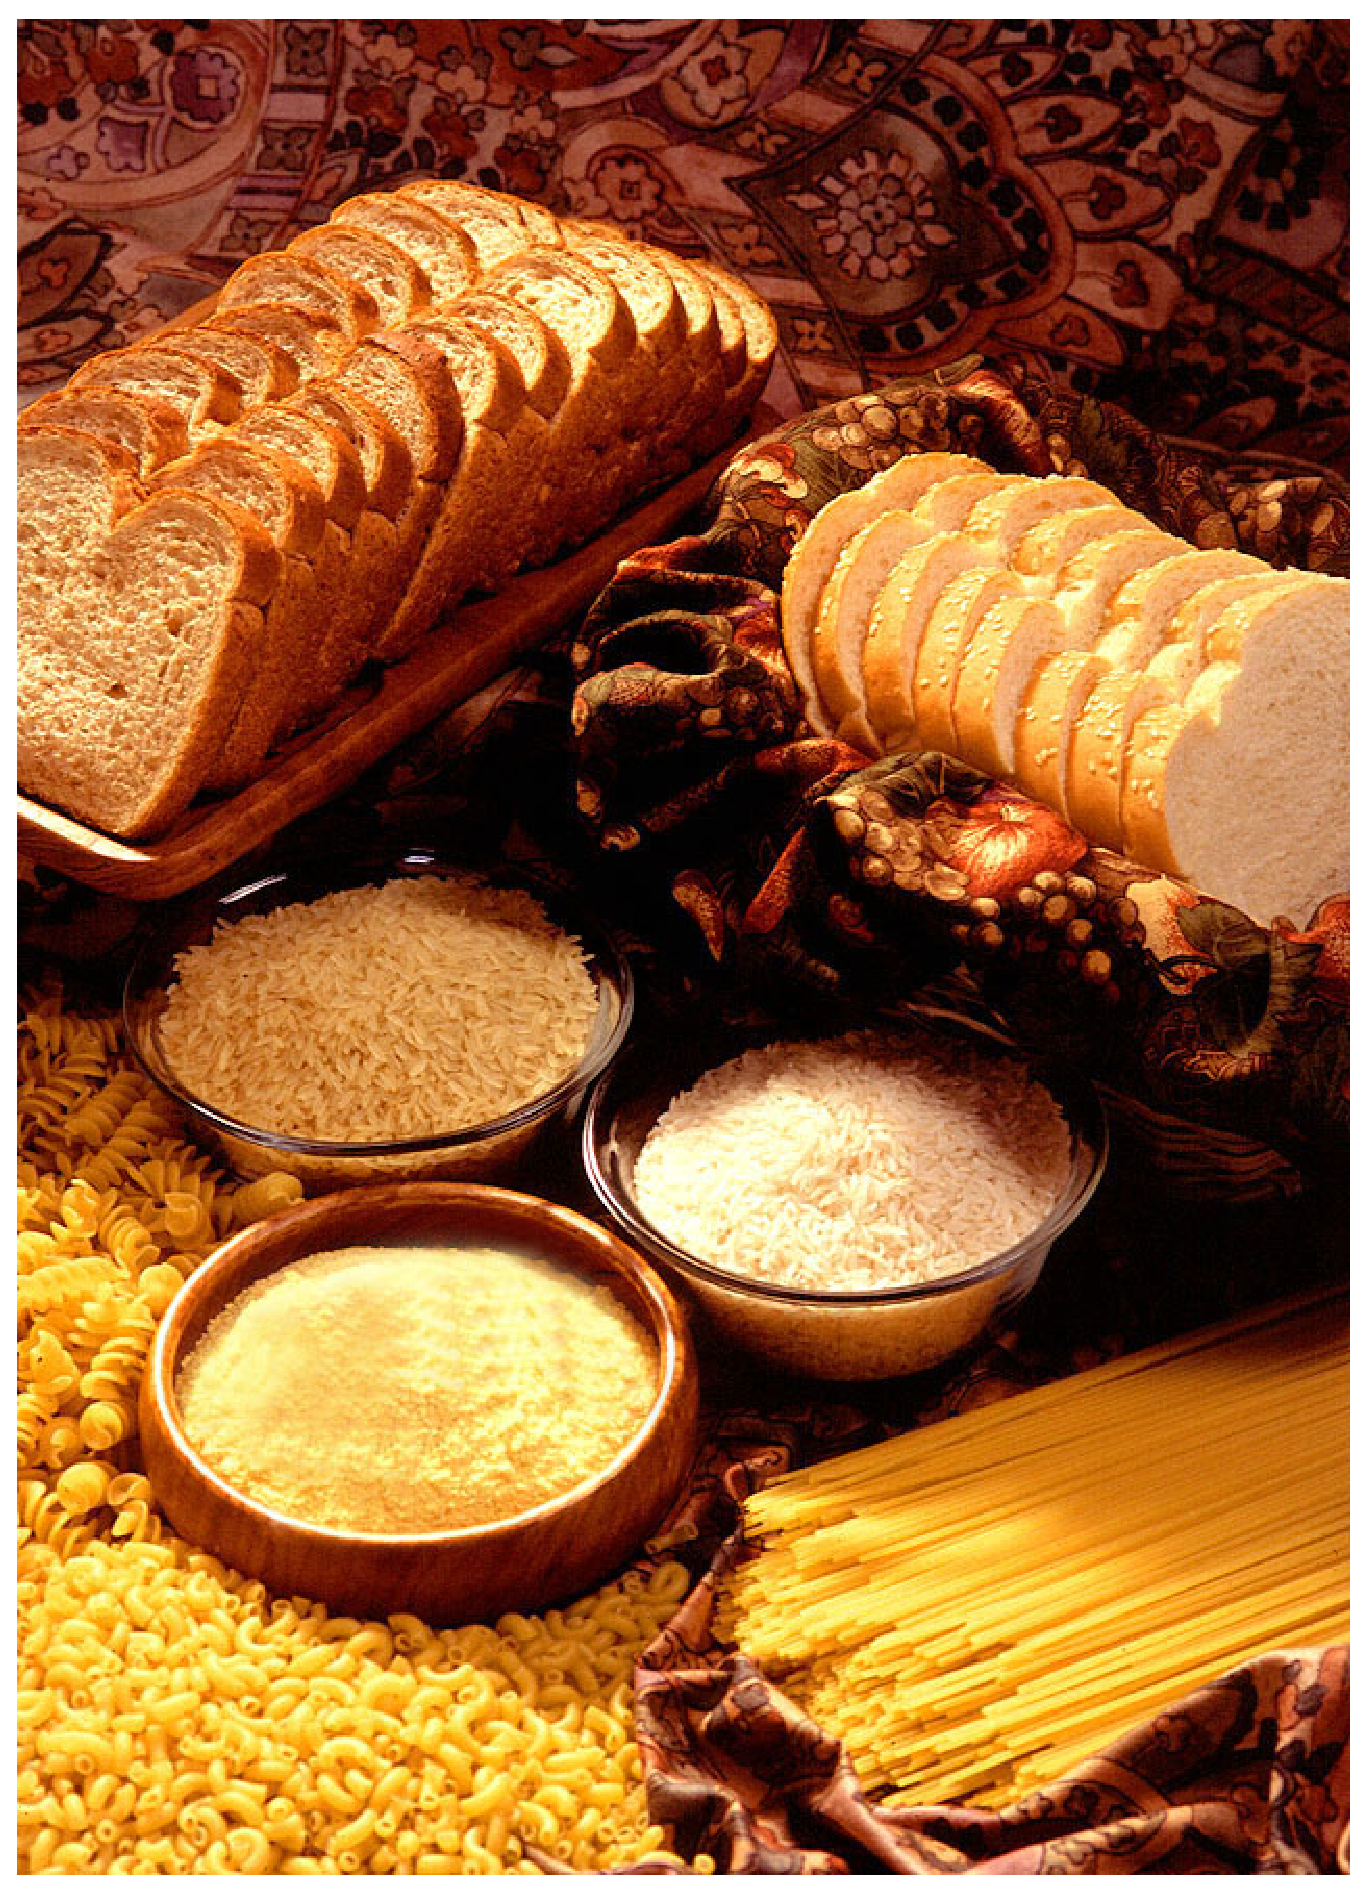
\includegraphics[width=7cm]{starchy-foods}
  \caption{Foods rich in carbohydrates~\cite{PicCarbohydrates}}
\end{figure}


Carbohydrates\index{carbohydrate} (also called saccharides) are the most important sources of fuels for the human body, by amount.
Especially the brain is highly dependent on carbohydrates as fuel sources, given that it can't combust fats, contrary to muscles.
One gram of carbohydrates provides 4 kcal (17 kJ) of energy, one ounce 113 kcal or 482 kJ.
The human body can build all carbohydrates from proteins and glycerol, a constituent of fat, so therefore are carbohydrates not essential.
Nevertheless should the sufficient supply of carbohydrates be part of the daily food intake.
Else there's a risk that valuable proteins of the body are depleted (for instance muscles).
An excess of carbohydrates can be stored on a short term base in the liver (\sfrac{1}{3}) and in the muscle tissue (\sfrac{2}{3}) in the form of glycogen.
The carbohydrate storage capacity is very small, as opposed to the fat storage capacity, which is almost limitless.
These carbohydrate reserves are getting tapped into when a fast straining performance is required, for instance flight from an enemy.
In an untrained person, they are enough for about 45 minutes of endurance running.
If our body gets more carbohydrates than necessary for maintaining the energy, the excess gets transformed into fats and stored in the form of body fats.

Carbohydrates (or saccharides) have the following characteristics:
\begin{itemize}
\item important source of energy for the cells
\item being able to be stored in liver and muscles in the form of glycogen\index{glycogen}\index{storage!sugar} on a short term base
\item maintaining the body temperature
\end{itemize}

\subsection{Structure of Carbohydrates}

The term carbohydrates\index{carbohydrate} comes from the chemical composition of this food constituent.
They are \emph{carbon} chains which are connected to water molecules, $H_2O$, (\emph{hydrate}d).
Carbohydrates can be separated onto the following categories:
\begin{description}
\item[digestible carbohydrates] like sugar and starch
\item[non--digestible carbohydrates] like fibers\index{fiber} (see chapter fibers, chapter~\ref{chap:fibers}, p.~\pageref{chap:fibers})
\end{description}

The carbohydrates are composed from the basic building blocks, the saccharides (sugar).
We distinguish monosaccharides, disaccharides, oligosaccharides and polysaccharides, with one, two, multiple or many sugar units respectively.

\subsection{Fast and Slow Carbohydrates}
\end{document}